% Stanford University PhD thesis style -- modifications to the report style
% This is unofficial so you should always double check against the
% Registrar's office rules
% See http://library.stanford.edu/research/bibliography-management/latex-and-bibtex
% 
% Example of use below
% See the suthesis-2e.sty file for documentation
%
\documentclass{report}
\usepackage{suthesis-2e}
\usepackage{hyperref}
\usepackage{natbib}
\usepackage{times}
\usepackage{amsmath}
\usepackage{amssymb}
\usepackage{amsthm}
\usepackage{booktabs}
\usepackage{graphicx}
\usepackage{subcaption}
\usepackage{multirow}
\usepackage{algorithm}
\usepackage{algorithmic}
\usepackage{ifthen}
\usepackage{color}
\usepackage[utf8]{inputenc}
\usepackage{url}
\usepackage{booktabs}

\input std-macros
\input macros

\dept{Computer Science}
\begin{document}
\title{Debiasing natural language evaluation with humans in the loop and statistical estimators}
\author{Arun Tejasvi Chaganty}
\principaladviser{Percy S. Liang}
\firstreader{Christopher D. Manning}
\secondreader{Michael S. Bernstein}
%\thirdreader{Jane Supernumerary} %if needed
%\fourthreader{Severus Snape} %if needed
 
\beforepreface{}
\prefacesection{Preface}
In natural language tasks such as knowledge base population, text summarization or open-response question answering, a significant challenge is simply evaluating the performance of automated systems because of the large diversity of possible outputs.
% ^^ Include the fact that the domain has shifted?
Existing fully-automatic methods for evaluating these systems rely on an \textit{incomplete} set of annotated references which lead to \textit{systematic biases} against certain system improvements: in other words, genuinely good ideas are systematically discarded simply because of limitations in our evaluation methodology.
As a result, human evaluation, which can be prohibitively expensive, has remained the most trusted mode of evaluation for these tasks.
In this work, we show how one can decrease the costs of incorporating human feedback through the design of appropriate statistical estimators. 
% JARGON: contrast between tasks which are very straightforwards.
%
% Some tasks are very clear cut: classification, parsing, question answering.
% others we really don't know what we're doing.

First, we consider the \textit{``finite incompleteness''} setting where the output space is too large to exhaustively annotate, but we may still expect significant overlap between the output of different systems. 
Naively combining annotations from different systems leads to a representation bias.
Here, we show that the cost of obtaining human feedback can be significantly amortized by using a novel importance-reweighted estimator.  
We apply this estimator to design a new evaluation methodology for knowledge base population and empirically show that the cost of evaluating precision and recall within this framework can be reduced by a factor of 4.

Next, we consider the \textit{``infinite incompleteness''} setting wherein few, if any, systems ever produce identical output.
Traditionally, the community has relied on similarity-based automatic metrics such as BLEU or ROUGE to compare the outputs produced by different systems.
Unfortunately, these metrics have been shown to correlate poorly with human judgment and thus introduce bias in evaluation.
We derive an unbiased estimator that optimally combines these automatic metrics with human feedback.
Our theoretical results allow us to characterize potential cost reductions only in terms of the tasks' subjectivity, measured by inter-annotator variance, and the automatic metrics' quality, measured by correlation with human judgments.
On two popular natural language generation tasks, question answering and summarization, we empirically show that currently we can achieve at most a 7--13\% reduction in cost on two tasks, exposing fundamental limitations in \hyphenation{de-biasing} current automatic metrics.

Finally, we turn our attention to \textit{incompleteness in the training data}, particularly in low-resource settings.
Here, our machine learning systems simply have not seen sufficient training data for a particular phenomenon to accurately make predictions for them at test time. 
To tackle this incarnation of incompleteness, we train a system ``on-the-job'' by requesting for human feedback in real-time while the model is deployed to economically fill in holes in the training data and thus resolve uncertainty in the model.
Our key idea here is to cast the problem as a stochastic game based on Bayesian decision theory, which allows us to balance latency, cost, and accuracy objectives in a principled way.
When tested on three classification tasks---named-entity recognition, sentiment classification, and image classification---we obtain an order of magnitude reduction in cost compared to full human annotation even when starting from zero training examples, while also boosting performance relative to a classical supervised model on the expert-provided labels.

\prefacesection{Acknowledgments}
I would like to thank\dots

\afterpreface{}

\section{Introduction}
\label{sec:intro}

\begin{figure}[t]
  \centering
  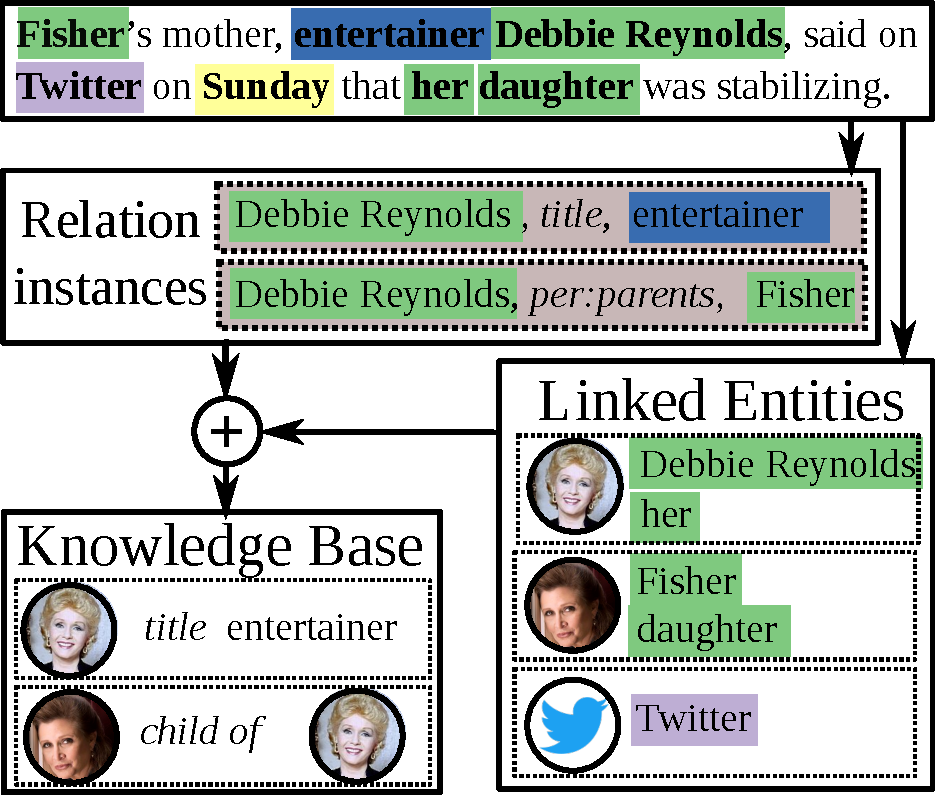
\includegraphics[width=0.6\columnwidth]{figures/entities-example.pdf}
  \caption[Example: KBP]{\label{fig:example} An example describing entities and relations in knowledge base population.}
\end{figure}

% (1 page w/ figure)
% Goal: remind the reader what information extraction is, what its relation to knowledge base population is and why it is important. Hook question.
Harnessing the wealth of information present in unstructured text online has been a long standing goal for the natural language processing community.
In particular, knowledge base population seeks to automatically construct a knowledge base consisting of relations between entities from a document corpus. % (\reffig{example}).
Knowledge bases have found many applications including question answering \citep{berant2013freebase, fader2014open,reddy2014large}, automated reasoning \citep{kalyanpur2012structured} and dialogue~\citep{han2015exploiting}.

% Evaluation @ scale poses problem. -- pooling methodology
Evaluating these systems remains a challenge as it is not economically feasible to exhaustively annotate every possible candidate relation from a sufficiently large corpus.
As a result, a pooling-based methodology is used in practice to construct datasets, similar to them methodology used in information retrieval \citep{sparck1975report, harman1993trec}.
For instance, at the annual NIST TAC KBP evaluation, all relations predicted by participating systems are pooled together, annotated and released as a dataset for researchers to develop and evaluate their systems on.
However, during development, if a new system predicts a previously unseen relation it is considered to be wrong even if it is correct.
The discrepancy between a system's true score and the score on the pooled dataset is called \emph{pooling bias} and is typically assumed to be insignificant in practice~\citep{zobel1998reliable}.

% Key finding: pooling bias
The key finding of this paper contradicts this assumption and shows that the pooling bias is actually significant, and it penalizes newly developed systems by 2\% \fone{} on average (\refsec{kbpo:analysis}).
Novel improvements, which typically increase scores by less than 1\% \fone{} on existing datasets, are therefore likely to be clouded by pooling bias during development.
Worse, the bias is larger for a system which predicts qualitatively different relations systematically missing from the pool.
% anti-solution
Of course, systems participating in the TAC KBP evaluation do not suffer from pooling bias, but this requires researchers to wait a year to get credible feedback on new ideas.
% TODO: I would like to add something about how ML methods are hosed, but perhaps for later?
% Chris's comment:  - Not addressed by Zobel, but I feel there is a big difference between whether this bias is a problem when used just for evaluation or also for system training (machine learning). If just for evaluation, some bias is a shame but doesn’t really badly effect things. If you are training systems assuming that your result set is the complete set of positives, then I feel that the effect of this bias is much more harmful, and this is the part that really impedes progress.

This bias is particularly counterproductive for machine learning methods as they are trained assuming the pool is the complete set of positives.
Predicting unseen relations and learning novel patterns is penalized.
The net effect is that researchers are discouraged from developing innovative approaches, in particular from applying machine learning, thereby slowing progress on the task. 

%These observations may explain why rule-based systems still play such a significant role in the top submissions at TAC KBP, and why, even after 8 years, top automated systems achieve scores of only about 35\% \fone{} while human annotators score above 60\% \fone{} on the same task.

% Solution: on-demand evaluation.
Our second contribution, described in \refsec{method}, addresses this bias through a new evaluation methodology, \emph{on-demand evaluation},
which avoids pooling bias by querying crowdworkers,
while minimizing cost by leveraging previous systems' predictions when possible.
%When a researcher submits a new system's predictions to our evaluation platform,
%we carefully sample a subset of its predictions and have crowdworkers judge them.
%just enough of its predictions to guarantee an accurate estimate of scores and have crowdworkers judge them.
We then compute the new system's score based on the predictions of past systems using importance weighting.
As more systems are evaluated, the marginal cost of evaluating a new system decreases.
% Experimental results.
We show how the on-demand evaluation methodology can be applied to knowledge base population in \refsec{application}.
Through a simulated experiment on evaluation data released through the TAC KBP 2015 Slot Validation track, we show that we are able to obtain unbiased estimates of a new systems score's while significantly reducing variance.

Finally, our third contribution is an implementation of our framework as a publicly available evaluation service at \url{https://kbpo.stanford.edu}, where researchers can have their own KBP systems evaluated.
The data collected through the evaluation process could even be valuable for relation extraction, entity linking and coreference, and will also be made publicly available through the website.
We evaluate three systems on the 2016 TAC KBP corpus for about \$150 each (a fraction of the cost of official evaluation).
We believe the public availability of this service will speed the pace of progress in developing KBP systems.


\appendix

\bibliographystyle{plain}
\bibliography{all}
\end{document}
